\documentclass{standalone}
\usepackage{tikz}
\usepackage{ctex,siunitx}
\usepackage{tkz-euclide}
\usepackage{amsmath}
\usetikzlibrary{patterns, calc}
\usetikzlibrary {decorations.pathmorphing, decorations.pathreplacing, decorations.shapes,}
\begin{document}
\small
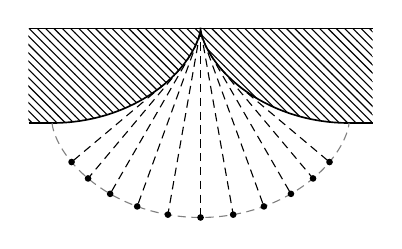
\begin{tikzpicture}[>=latex,scale=0.6,inner sep=1pt]
  \draw[semithick,domain=-180:180,samples=200] plot ({\x/180*pi-sin(\x)},{cos(\x)-1});
  \draw[semithick](-0.5-pi,0)--(0.5+pi,0);
  \draw[semithick](-0.5-pi,-2)--++(0.5,0);
  \draw[semithick](pi,-2)--++(0.5,0);
  \fill[semithick,domain=-180:180,samples=200,pattern=north west lines] plot ({\x/180*pi-sin(\x)},{cos(\x)-1})--++(0.5,0)--++(0,2)--++(-1-2*pi,0)--++(0,-2)--cycle;
  \draw[densely dashed,gray,domain=0:360,samples=200] plot ({\x/180*pi-pi-sin(\x)},{cos(\x)-3});
  \foreach \x[count=\i] in {-100,-80,...,100}
  {
    \draw[densely dashed] ({\x/180*pi-sin(\x)},{cos(\x)-1})--++({270+\x/2}:{4*cos(\x/2)})coordinate(\i);
    \fill(\i) circle(2pt);
  }
\end{tikzpicture}
\end{document}